\chapter{Resultados y Análisis}

\section{Software}

Se desarrolla la aplicación web de manera local, y posteriormente se lanza a la web, esta compuesta por los siguientes sitios y las diferentes interacciones basadas en las funciones basicas, crear, leer, actualizar y borrar (CRUD).

\begin{itemize}
	\item Parte Pública
	\item Parte Privada
	\begin{itemize}
		\item API
		\item Panel de Control
		\begin{itemize}
			\item Crear
			\item Ver
			\item Editar
			\item Eliminar 
		\end{itemize}
	\end{itemize}
\end{itemize}

De acuerdo a la lista anterior, se toman en cuenta dos partes para esta, una pública y una privada, como se observa en la figura \ref{fig:index}. En la parte pública se encuentra una vista con los datos de contacto, solicitudes de registro o productos y la cantidad de usuarios que actualmente estan registrados en la aplicación. En la parte privada se encuentra la interacción de los usuarios sea administrador, dueño de una casa o de una habitación, para controlar y ver sus datos.\\

Las diferentes interacciones que tiene cada usuario en el panel de control se garantizan por medio del framework, creando diferentes roles para cada usuario que se esta registrando y realizando la comprobación por parte de los controladores y el middleware que este provee.

\begin{figure}[H]
\centering
\caption{Página de Inicio}
\label{fig:index}
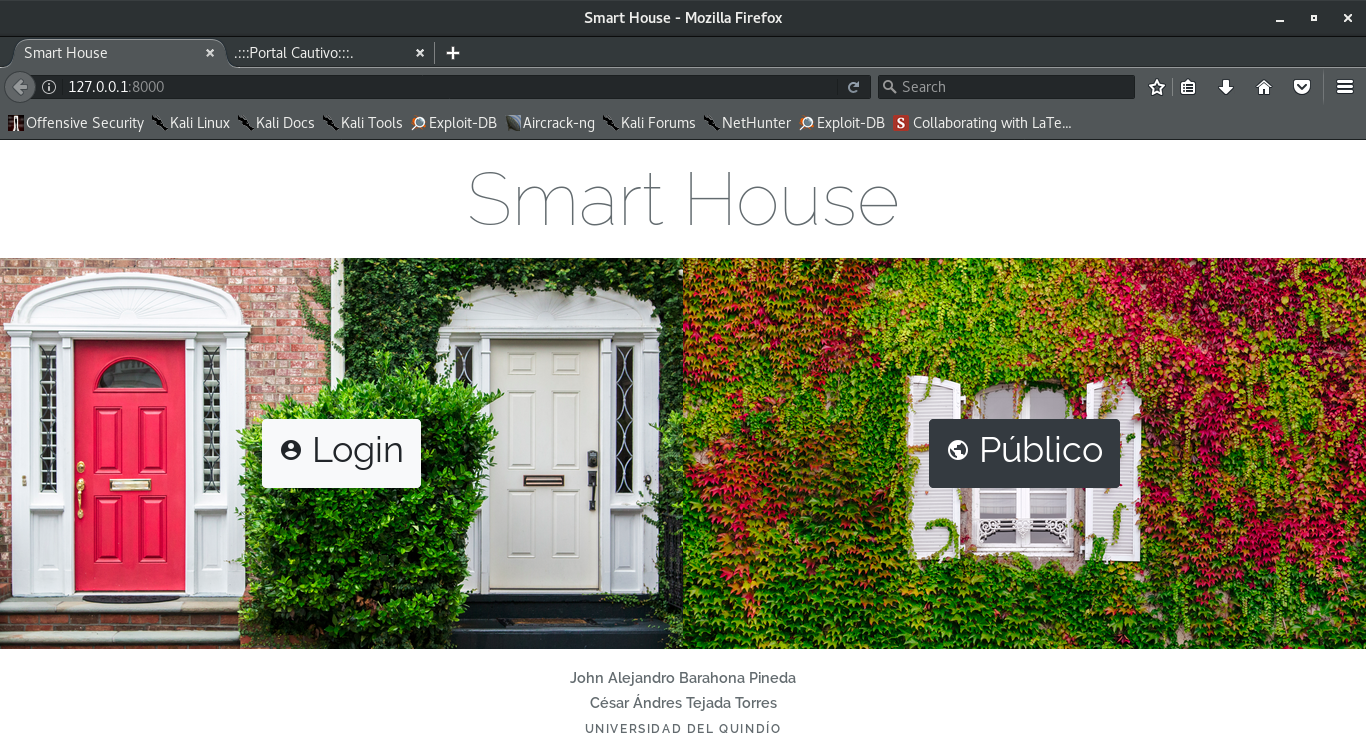
\includegraphics[width=0.9\linewidth]{Imagenes/Index}
\end{figure}

\subsection{Parte Pública}

En esta vista unicamente hay opciones para el contacto y solicitudes, como se menciona anteriormente, es una vista sencilla dada la poca información que contiene, como se observa en la figura \ref{fig:publicview}.

\begin{figure}[H]
\centering
\caption{Vista Pública}
\label{fig:publicview}
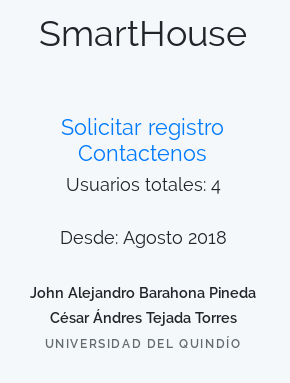
\includegraphics[width=0.9\linewidth]{Imagenes/Public_view}
\end{figure}

\subsection{Parte Privada}

En esta sección es donde se encuentra el Panel de Control para los diferentes usuarios de la aplicación. En primera instancia, para un usuario administrador, que es el encargado de gestionar la aplicación, este usuario tiene la posibilidad de crear, ver, editar y eliminar los diferentes registros de la aplicación, la vista de este usuario se puede observar en la figura \ref{fig:adminview}. Por medio de este usuario es que se activan las cuentas de los demás, por esto en la parte pública estás las opciones de contacto y solicitud de registro.\\

\begin{figure}[H]
	\centering
	\caption{Vistas de Usuarios}
	\label{fig:views}
	\subfigure[Usuario Administrador]{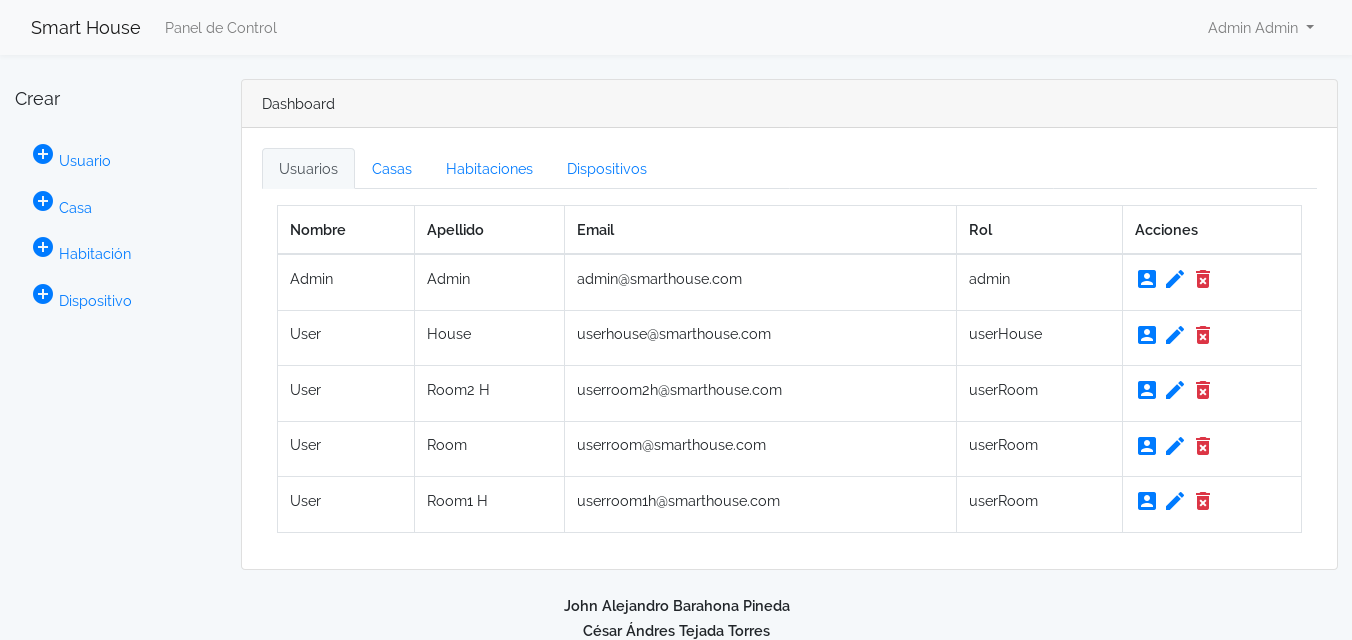
\includegraphics[width=0.9\linewidth]{Imagenes/Admin_view}
		\label{fig:adminview}}
	\subfigure[Usuario de Casa]{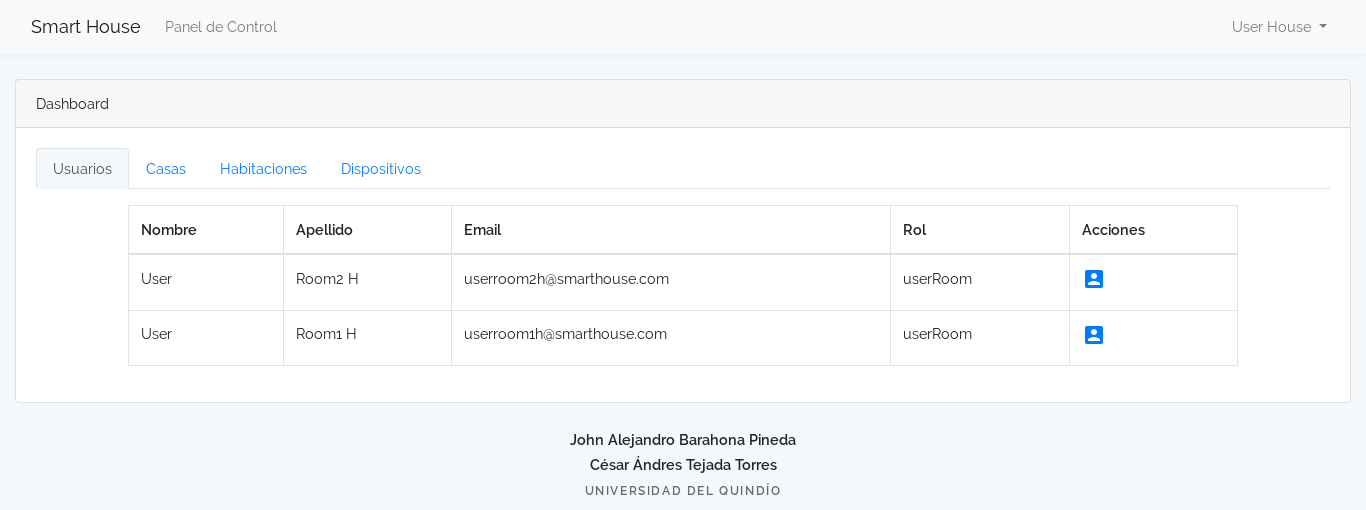
\includegraphics[width=0.45\linewidth]{Imagenes/UserH_view}
		\label{fig:userhview}}
	\subfigure[Usuario de Habitación]{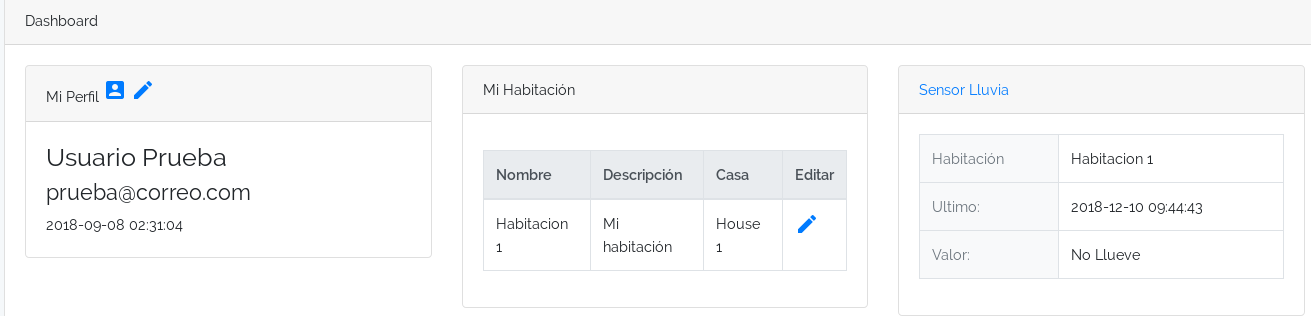
\includegraphics[width=0.45\linewidth]{Imagenes/UserR_view}
		\label{fig:userrview}}
\end{figure}


También existe el usuario dueño de la casa donde se encuentra el dispositivo, este usuario es opcional y es para gestionar los dispositivos presentes dentro de una misma casa, es un administrador de la casa, el cual puede ver y editar algunos campos de sus usuarios hijos o usuarios habitación y sus diferentes casas y habitaciones, unicamente las que esten registradas a su nombre, como se ve en la figura \ref{fig:userhview}, de este modo el rol de este usuario es administrar su casa y visualizar los datos de esta.\\

Por último, otro rol es el de usuario habitación, el cuál es un usuario que solo visualiza sus propios datos, como la habitación y los dispositivos presentes en esta, como se observa en la figura \ref{fig:userrview}, a este solo le compete la información de lo que posee en su habitación, por tal motivo el panel de control muestra una vista general de los datos y el estado de sus dispositivos, además de tener la capacidad de editar partes básicas de su habitación y perfil. Este usuario puede o no estar sujeto a un usuario padre o usuario casa, ya que, solamente puede poseer una tarjeta para su habitación y ninguna otra en dicha casa.\\

	

Además de este panel de control, desde el cuál se realizan las operaciones sobre la aplicación, en la parte privada se encuentra la ruta encargada de la actualización Servidor-Tarjeta, es decir, en esta ruta es donde se da la comunicación. En esta ruta se realiza una petición HTTP tipo GET por parte de la tarjeta, esta contiene el id de la habitación en la cuál esta instalada la tarjeta y también el token correspondiente a esta, y además en la URL se añade un texto tipo JSON en el cual se encuentra toda la información de la lectura actual de los sensores, esta petición la responde el servidor con un texto, también tipo JSON que contiene la información pertinente de las cargas o actuadores, como se observa la figura \ref{fig:updateview}, para dar seguridad a esta transacción, se se utiliza el token mencionado anteriormente, el cual se verifica mediante el id de la habitación y que este coincida con los datos almacenados, de este modo se garantiza que lo que se envía este sometido a verificación.

\begin{figure}[H]
\centering
\caption{Página de intercambio de datos}
\label{fig:updateview}
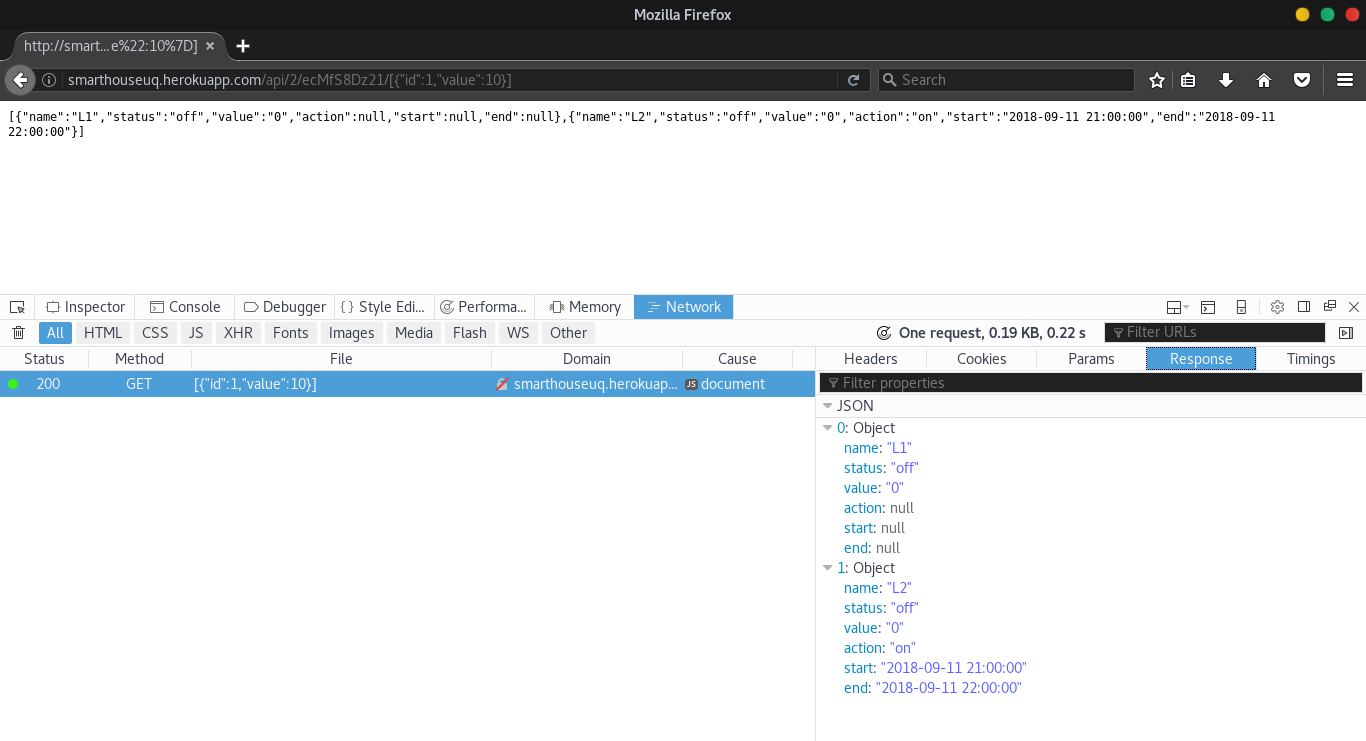
\includegraphics[width=0.9\linewidth]{Imagenes/Update_view}
\end{figure}


\subsection{Base de Datos}

La estructura de la base de datos se puede observar en la figura \ref{fig:db}, aquí se observan los diferentes campos que posee cada tabla, además de las llaves y sus relaciones, las relaciones presentes en esta estructura son de tipo 1:N, es decir, por ejemplo un usuario puede tener relacionadas N casas.

\begin{figure}[H]
\centering
\caption{Base de datos SmartHouse}
\label{fig:db}
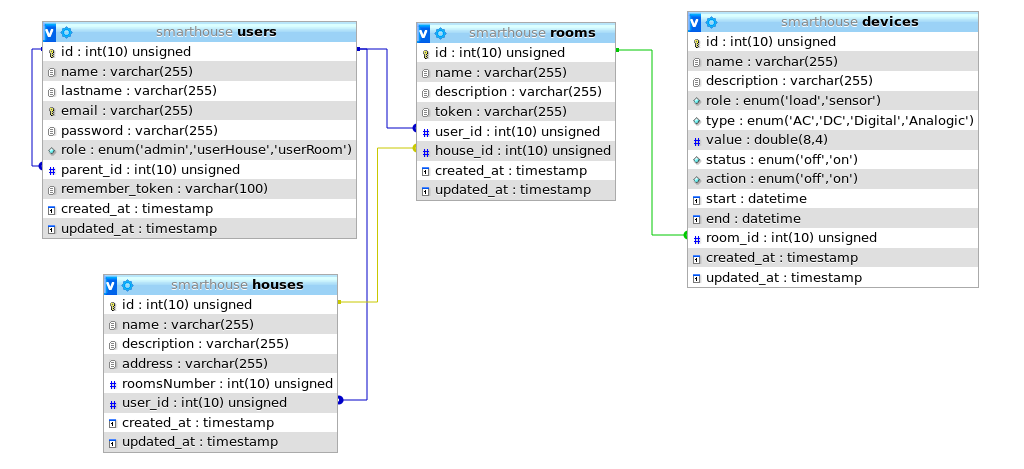
\includegraphics[width=0.7\linewidth]{Imagenes/DB}
\end{figure}

\section{Firmware}

\subsection{Conexión a Internet vía Wi-Fi}

Los sistemas IoT deben estar conectados siempre a Internet, por este motivo se debe brindar un canal para decirle al sistema como acceder a este, por lo tanto, se desarrolla una tarea que se encarga de esto, como se ha mencionado el módulo del esp32 es capaz de funcionar como Punto de Acceso (AP) y como Cliente o Estación (STA) al mismo tiempo, aprovechando esta capacidad se usa un servidor local, el cual se encarga de gestionar la conexión de la tarjeta con Internet.\\

De este modo, como se observa en la figura XXX esta es la pagina principal del servidor local de la tarjeta, la cual permite conectarse a una red que este al alcance de la tarjeta, y también desconectarse de esta, su funcionamiento es muy intuitivo, se selecciona la red a la que se desea conectar la tarjeta, se ingresan sus credenciales y posteriormente el dispositivo verifica si la conexión fue exitosa o no, si la conexión es exitosa ya la tarjeta esta lista para su funcionamiento, basta con reiniciarla para que solo quede funcionando como STA y no en el modo dual, además de esto si las credenciales de la red cambian también se incluye un botón para el borrado de estas, de este modo se puede configurar de nuevo una red.

\subsection{Escritura de Datos en la Aplicación Web}

Los datos que esta leyendo la tarjeta provienen de los diferentes sensores que tiene conectados como se ha mencionado, se usan sensores de estado para sensar la presencia, sensor de calidad de aire entre otros presentes en esta. Para la escritura de los datos, en el firmware, se desarrollan diferentes tareas encargadas de leer y enviar los datos a una tarea central, los datos que están enviando contienen el id del dispositivo y la medida que lee en ese momento, estos datos se envian en forma de texto en formato JSON, de este modo, la tarea central los gestiona y envía a la aplicación con el mismo formato, organizandolos en la petición HTTP tipo GET que realiza. La aplicación ya se encarga de almacenarlos y mostrarlos al usuario como se menciona anteriormente.

\subsection{Lectura de Datos de Internet}

Al inicio de la aplicación, se sincroniza y se almacena la hora actual de la red, por medio del protocolo SNTP, esto con el propósito de poder gestionar las diferentes reglas solicitadas por el usuario, por ejemplo, que encienda o apague un dispositivo a una hora dada, después de obtener este dato la aplicación continua con normalidad para realizar las diferentes peticiones a la aplicación web.\\

La interacción del usuario se da con la aplicación web mencionada anteriormente, de este modo la tarjeta siempre se debe actualizar, para esto, cuando la tarjeta envía los datos de los sensores la aplicación responde con los datos necesarios para tarjeta, esta los recibe en una cadena texto en formato JSON, los procesa y los envía a las tareas pertinentes ya sea para encender o apagar algún dispositivo conectado a la tarjeta, además envía las reglas que el usuario ha definido.